\section{A public timetable: feasible fleets and bounded costs}\label{sec:public}

The exact two-service example isolates the mechanism; it does not measure
its prevalence or size in service.  For a timetable-scale check we use the
published Hildenbrand instance from the Sistig electric-bus scheduling data
\citep{sistig2025dataset,sistig2025electrification}: 37 mandatory services
with a complete directed deadhead matrix.  We form
two \emph{separate} one-depot cases, using depot 15 or depot 16.  These are
declared modifications of the source network, not a reconstruction of its
two-depot, multiple-output charging design.  Timetable and directed travel
times retain their source offsets, including the next-day services.  Matrix
travel times depend on origin and destination, not on departure time.

Energy and monetary inputs are explicit scenario assumptions, not observed
vehicle telemetry or source objective coefficients.  Service energy is
$1.20$ kWh/km plus 16 kWh per service hour.  Directed deadheads use
$0.96$ kWh/km plus 16 kWh per travel hour, and explicit off-depot waiting
uses 16 kWh/h; depot-parked auxiliary draw is zero.  Each used bus has
400 kWh usable inventory, zero additional reserve, unit charging
efficiency, and a 360 kW acceptance limit.  One 360 kW connector is shared
at the selected depot.  All used buses start full and return full by a
synthetic 30:00 service-block boundary.  Charging has no taper and no
switching time.  This finite block does not establish a repeating daily
operation.  A 37-bus one-service-per-bus construction confirms feasibility
of both cases, but has no optimization role.  Monetary travel cost is zero:
the objective charges the used-bus fee and grid energy, while movement
energy and time remain in the physical constraints.

We first use synthetic used-bus cost $f=100$ and flat grid price
$a=0.2$ per kWh.  Because this objective is linear in load, minimizing it
over the hull of complete plans has the same value as minimizing it over
physical plans; this flat-price experiment cannot exhibit a physical--hull
gap.  The original fixed-budget native runs returned physically replayed
two-bus schedules in both depot cases without proving objective optimality.
A separate, already archived round-0 solve
within the later nonlinear planner used the same complete depot-15 physical
case and a tangent objective that reduces exactly to the flat price.
That call returned a \emph{native numerical} optimum of approximately
408.53, with matching incumbent and lower bound under solver tolerances.
This is a retrospective interpretation of one call, not a new flat-price
experiment or a reclassification of the nonlinear campaign.  The numerical certificate does not identify the exact rational-model
optimum.  The following ideal stored-input certificates answer that
distinct exact-arithmetic question.

For both depot graphs, a one-bus path is impossible.  Chronologically
forced adjacent services leave no admissible depot visit, while mandatory
service energy alone exceeds one bus's 400 kWh inventory.
An exact cardinality-gated path-cover relaxation of each full 37-service
graph gives flat-objective lower bounds displayed outward as 404.92 at depot
15 and 414.39 at depot 16.  The bounds retain every declared connection
mode but relax some physical constraints.  Separately, an exact rational
depot-15 witness covers all 37 services with two buses, respects the shared
connector, and restores both batteries to 400 kWh by 30:00.  Hence depot 15's ideal
model has a minimum fleet of two and the \emph{flat-cost optimum} lies in
\begin{equation}\label{eq:public-flat}
 D^{\rm flat}_{15}\in[404.92,408.54]
 \quad\text{(outward-rounded exact rational bounds).}
\end{equation}
The bounds do not identify the optimum.  Depot 16 has the exact
at-least-two obstruction and lower bound, but its returned two-bus upper
witness remains numerical, yielding a mixed-evidence interval
$[414.39,433.75]$ after outward rounding.  In
particular, a native solver's rounded matrix and its feasibility tolerances
are distinct from the ideal stored-input rational model.

For a nonlinear illustration on \emph{the same finite depot-15 ideal
model}, let $e_t$ be hourly grid energy for 30 market intervals and set
\begin{equation}\label{eq:public-quadratic}
 F(e)=\sum_{t=1}^{30}\left(0.2e_t+\frac{e_t^2}{1800}\right).
\end{equation}
The coefficients and bus cost remain synthetic.  The exact two-bus witness
gives a physical upper bound displayed as 512.77.  To bound the complete
hull from below, let $L_{\rm flow}$ denote the exact depot-15 two-path
flat-cost relaxation value.  Because monetary travel cost is zero, it
implies at least $E_{\min}=(L_{\rm flow}-2f)/a\approx1024.62$ kWh for any
two-bus plan.  One bus is impossible, and a uniform-price comparison using
the service-energy floor excludes three-or-more-bus plans from improving the
dual lower certificate.  The 30-period Fenchel inequality then gives the
exact rational lower bound displayed as 424.36.  Therefore
\begin{equation}\label{eq:public-nonlinear}
 424.36\leq CH_{15}\leq D_{15}\leq512.77,
 \qquad 0\leq D_{15}-CH_{15}\leq88.41.
\end{equation}
All displayed endpoints are rounded outward from the exact bounds.  They
do not establish $CH_{15}$ or $D_{15}$ individually, nor a strictly positive
gap.  The public case thus demonstrates physically feasible complete-fleet
witnesses and useful bounds under declared assumptions, while leaving
public price support open.


\begin{figure}[t]
\centering
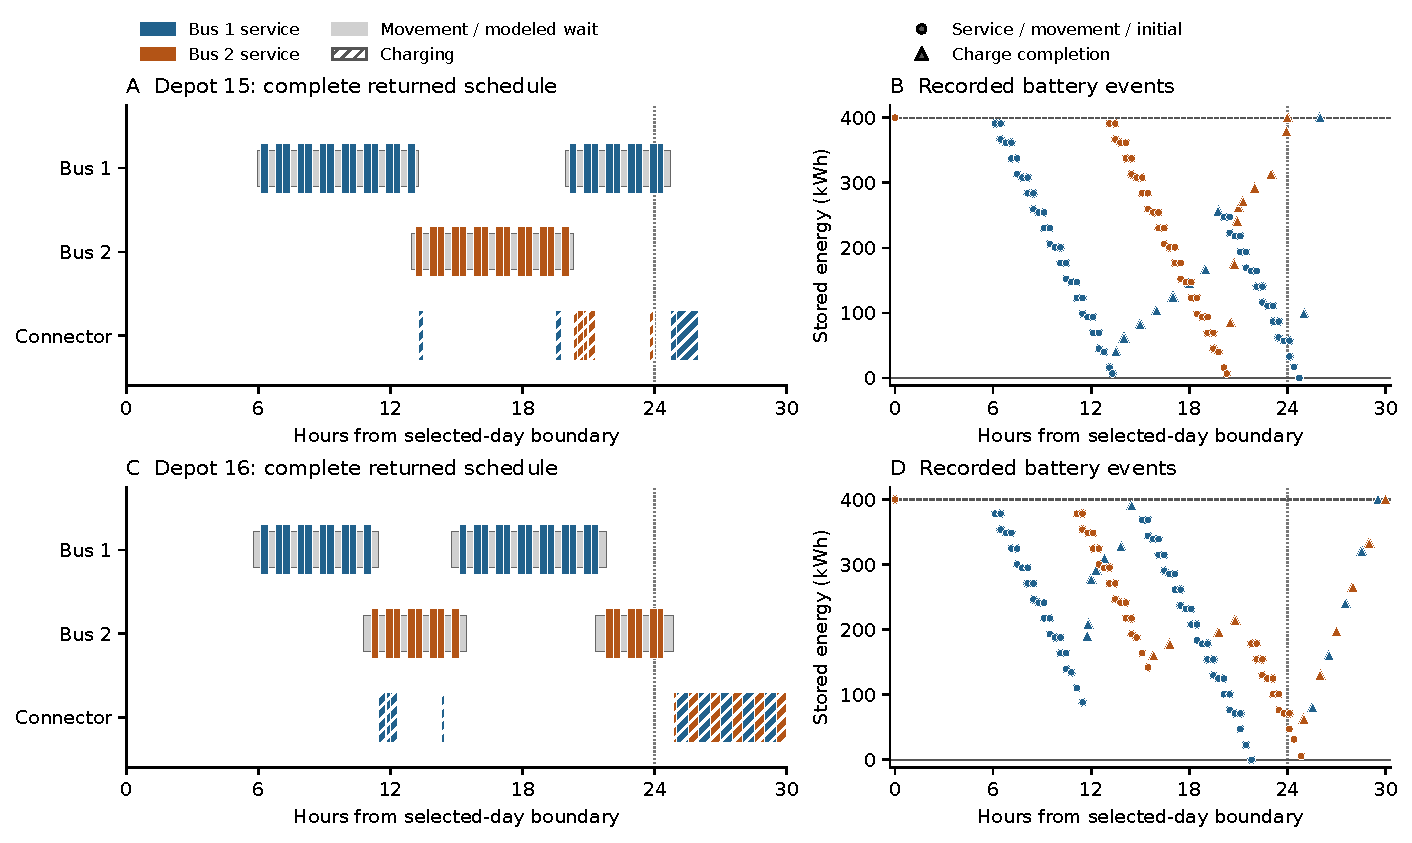
\includegraphics[width=\linewidth]{../figures/public_pilot_witnesses.pdf}
\caption{Two-bus schedules returned by the original flat-price pilot for
the two depot variants of the same Hildenbrand timetable.  Battery and
charging traces describe numerical feasible witnesses under the declared
scenario assumptions.  They are not measured operation, two independent
networks, or proofs of cost optimality.  The separately constructed exact
depot-15 witness supplies the ideal-model bounds in the text.}
\label{fig:public-witnesses}
\end{figure}
